\chapter{Experiment Description }

%%%%%%%%%%%%%%%%%%%%%%%%%%%%%%%%%%%%%%%%%%%%%%%%%%%%%%%%%%%%%%%%%%%%%%%%%%%%%%%%%%%
\section{The Large Hadron Collider}

The LHC is one of the most powerful particle collider in the world, it started construction in 1998 on the France–Switzerland border near Geneva, using the 26.7 km tunnel, constructed for the CERN LEP machine. It came into operation on the 10 of September of 2008, and it is the latest addition to the CERN accelerator complex. It was first approved on December 1994 by the CERN council, with  a center-of-mass-energy of 14 Tev \cite{Bruning:782076}.

The LHC consists of two separate rings, kept in an ultrahigh vacuum, where two the beams of particles are located. To achieve the circular motion of the beams, 1232 dipole magnets are used to maintain trajectory, and 392 quadrupole magnets are used to keep the beams focused. Near the interaction points, stronger quadruple magnets are used to increase the probability of interaction between the beams.  These magnets are made of coils of special superconductive cable, cooled to a temperature of 1.8 K with superfluid helium, producing an electromagnetic field of above 8 T \cite{Bruning:782076}.

 The beams in each ring are made of bunches for particles traveling near the speed of light. These bunches can be made of protons or ions (like lead nucleons), depending on the running experiment, however, the majority of events at the LHC are produced by proton-proton (pp) bunch collision.\\
A diagram of CERN’s accelerator complex can be seen in Figure \ref{cernc}. The proton bunches start as ionised hydrogen gas and are accelerated to an energy of 50 MeV, by the Linac 2 linear accelerator. Once they leave the Linac 2, they are further accelerated to an energy of 1.4 GeV by the Proton Synchrotron Booster (PSB) and dumped on the  Proton Synchrotron (PS). In the PS, the bunches are accelerated to an energy of 25 GeV and arranged into a bunch trains, with a spacing of 25 ns, in total, one orbit contains 3564 bunches, arranged in to several trains. Finally, the bunches pass from the PS to the Super Proton Synchrotron (SPS), where they are injected into the LHC with an energy of 450 GeV. In the LHC, the beams reach a peak energy of 6.5 TeV, and are made to collide in one of the 4 detectors, ALICE, ATLAS, CMS and the LHCb. 
\begin{center}
  \begin{figure}[ht]
    \centering
    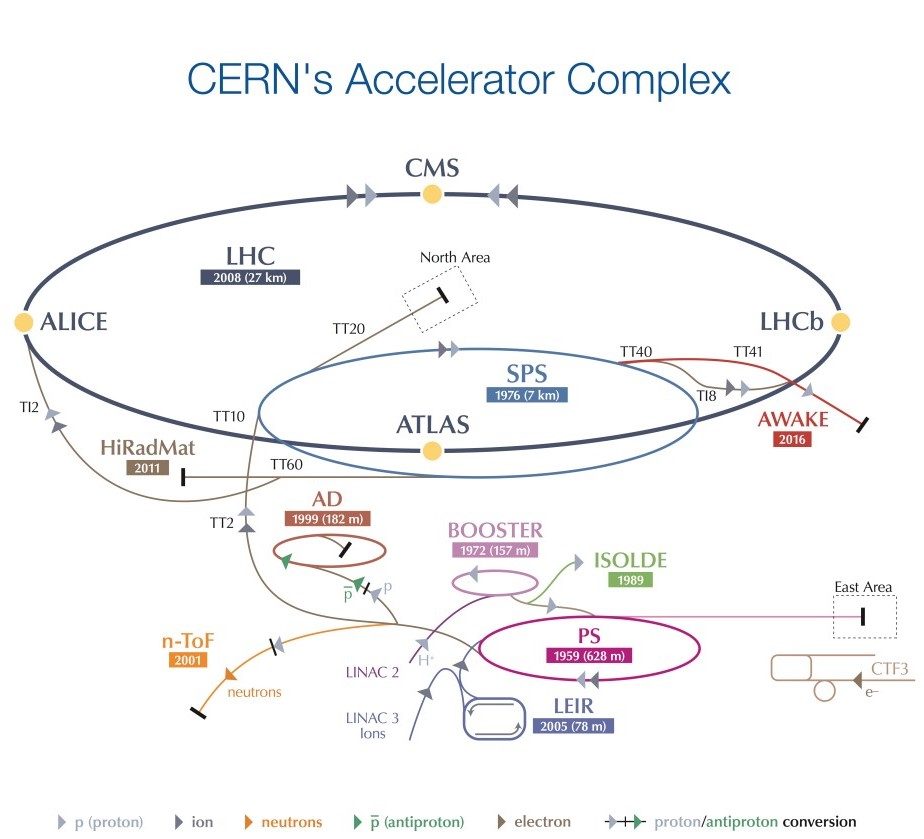
\includegraphics[scale=.7]{Chapter2/CERNC.jpg}
    \caption[CERN accelerator complex.]{A diagram of the CERN accelerator complex \cite{cernpg}.}
    \label{cernc}
  \end{figure}
\end{center}
The four detectors are tasked with measuring all the particles produced in pp collisions. Two specialized detectors are integrated to the LHC, ALICE and LHCb. ALICE is dedicated to heavy ion collisions physics, where the quark-gluon plasma is studied. The LHCb investigated the differences between matter and antimatter, by studying the “beauty quark” \cite{lhcb}.\\
The two remaining detectors, CMS and ATLAS, are general purpose detectors, tasked with studying a wide range of physics, from the search of the Higgs boson, to extra dimensions and particles that could make the dark matter in the universe \cite{cmsweb}.

Two operation runs have been completed so far at the LHC, and two long shutdowns, where maintenance and several minor upgrades were made to the machine.  Run 1 lasted from 2010-2012, while Run 2 lasted from  2015-2018. As of Run 2, the LHC has achieved a peak luminosity of $2\times 10^{-34} cm^{-2}s^-1$, two times the amount for which the LHC was designed. The integrated luminosity, since the LHC began operations, has reached $160 fb^{-1}$ for the ATLAS and CMS experiments \cite{lumi2180}.
%%%%%%%%%%%%%%%%%%%%%%%%%%%%%%%%%%%%%%%%%%%%%%%%%%%%%%%%%%%%%%%%%%%%%%%%%%%%%%%%%%%
\section{The CMS detector }
The Compact Muon Solenoid (CMS) experiment is one of the four major experiments currently running in the LHC, and along with ATLAS, one of the two high luminosity experiments at CERN. It receives its name from the huge solenoid magnet, from which the detector is built around. This solenoid takes the form of a coil made of super conductive wire, capable of producing an electromagnetic field of 4 T. The field is confined by a steal yoke, that weights 14,000 tones.

CMS is a layered detector, 21 m in length, with a height and width of 15 m, and it is composed of four main subdetectors, the inner silicon tracker, electromagnetic and hadron calorimeters and the muon detectors. The strong magnetic field produced by the detector’s solenoid, separates the particles produced in the coalitions and provides a better momentum resolution. Figure \ref{cms} shows a diagram of the detectors layout. 
\begin{center}
  \begin{figure}[ht]
    \centering
    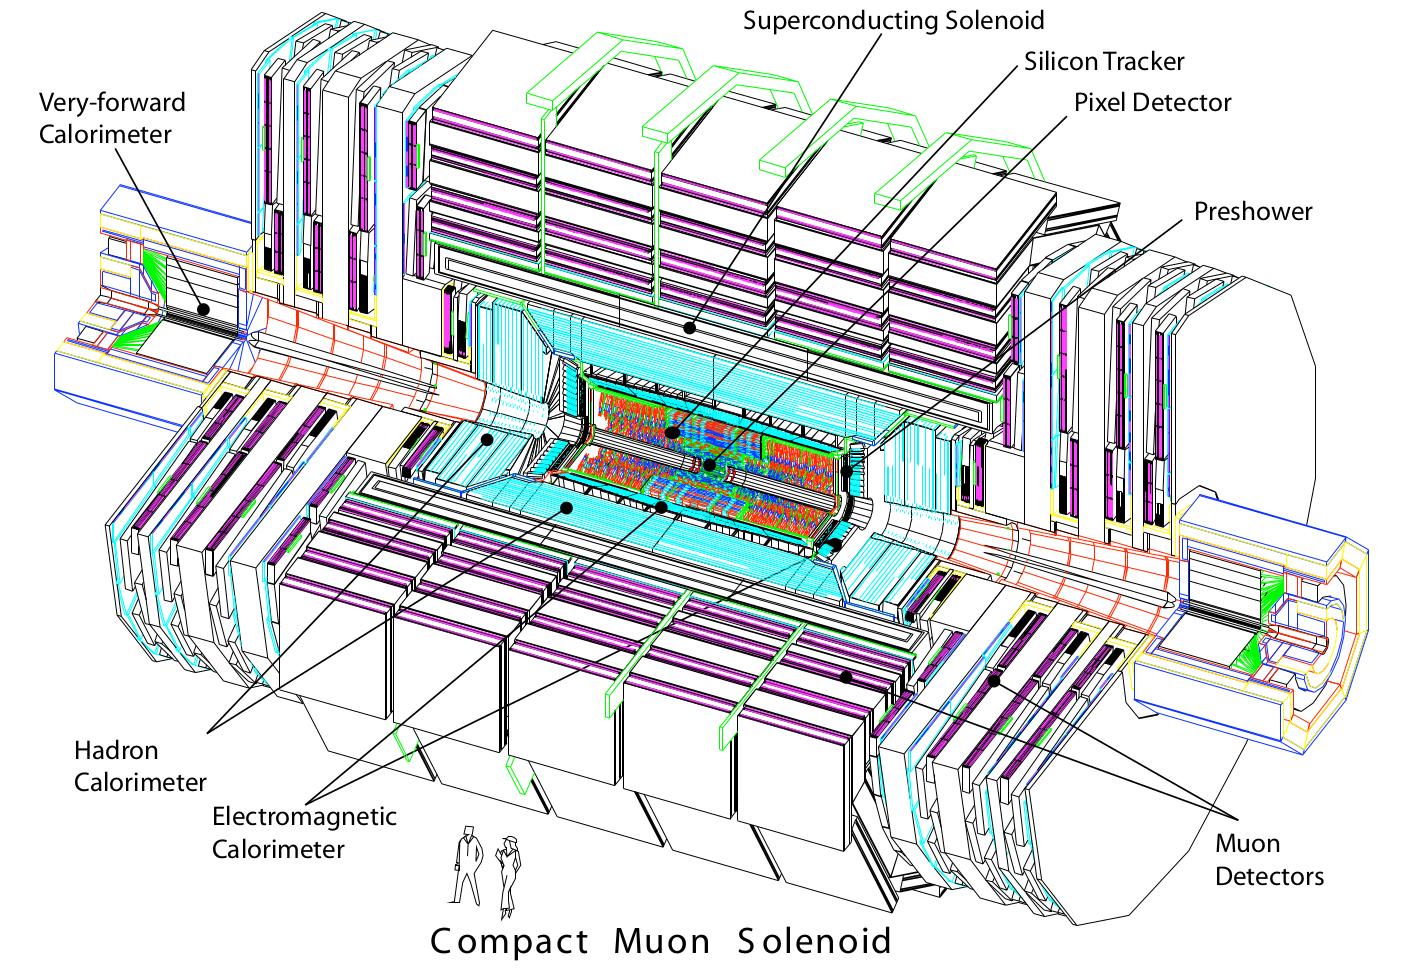
\includegraphics[scale=.2]{Chapter2/CMSl.png}
    \caption[CMS detector diagram]{Diagram of the CMS detector showing the various subdetectors that comprise it \cite{cms-manual}.}
    \label{cms}
  \end{figure}
\end{center}
The CMS experiment has a broad range of goals in particle physics, from studying the SM in search of new particles and phenomena, to searching for extra dimensions and discovering new particles that could make the dark matter in the universe.  The experiment has achieved great things in the scientific community, however, one of its greatest, was the discovery of the Higgs boson  alongside the ATLAS experiment in 2012. In the next subsection a brief description of the different subdetectors is provided \cite{cms-manual}.
\subsection{ Silicon tracker}
At the heart of the CMS detector lies the inner silicon tracker. As its name suggests, the purpose of this subdetector is to reconstruct the track of charged particles generated during collisions, by using silicon strips and pixels to register the paths of charged particles. Once the track of a charged particle is reconstructed, its momentum can be extracted, by calculating the curb of its trajectory, produced by the electromagnetic field. Also, the vertex, the origin of the track, can be determined. The Tracker, which consists of an Inner Tracker (pixels) and an Outer Tracker (strips), is the first subdetector encountered by the particles, and thus the smallest, with an outer radius of 110 cm and a total length of 5.4 m, Figure \ref{tracker} shows the layout of the inner tracker.
\begin{center}
\begin{figure}[ht]
    \centering
    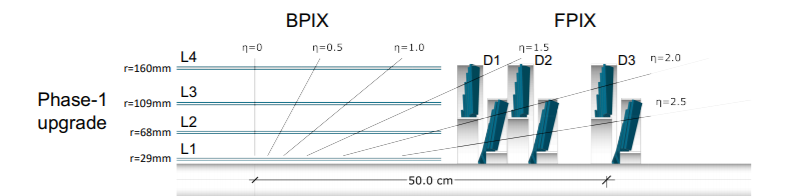
\includegraphics[width=1\textwidth]{Chapter2/pixel-detector.png}
    \caption[CMS tracker.]{Diagram showing the layout of the CMS Phase-1 inner tracker. The barrel pixel detector (BPIX) and the forward disks pixel detector (FPIX) are shown \cite{CMSTrackerGroup:2020edz}.}
    \label{tracker}
\end{figure}
\end{center}
The tracker is divided into two subtrackers: one is the silicon strip tracker, made of 9.6 million silicon strips. This subtracker is divided in two parts: the Tracker Inner Barrel (TIB) and the Tracker Outer Barrel (TOB). The TIB is made of 4 layers that cover up to $|z|<65$ cm. The TOB has 6 layers, and a coverage of $|z|<110$ cm. The encaps are again divided into two regions,  Tracker End Cap (TEC) and Tracker Inner Disk (TID). The TEC is composed of 9 disks that extend in the region 120 cm $<|z|<$ 280 cm, while the TID has 3 disks that fill the gaps in between the TIB and the TEC. The TEC and the TID are made of rings centered on the beam, and possess stripst that point towards the beam.\\
The strip tracker encompass and area of 200 $m^2$, and it is made of almost 15,400 modules, running at a  temperature of $-20^{\circ} C$.

The other subtracker is the pixel tracker, made of three layers of barrels possessing a radius of 4.4 cm, 7.3 cm and 10.2 cm with a length of  53 cm, and consisting of 66 million pixels.  In each end of the barrels, two  end cap disks reside, extending from 6 to 15 cm in radius and located at $|z|=34.5$ cm and 44.5 cm, in total, the pixel tracker has an area of roughly 1$m^2$\\
768 pixel modules are housed in the barrel, all arranged into half lathers of 4 identical modules. The end cap disks are designed in a turbine-like geometry, with blades rotated $20^{\circ}$. The blades are made of 7 different pixel modules, with a total of 768 modules being housed in the end cap disks \cite{cms-manual}.
\subsection{CMS calorimetry system}
The calorimetry system of the CMS detector is composed of two types of calorimeters: the electromagnetic and hadronic calorimeters. Both subdetectors form a complete and hermetic calorimetry system with a coverage of $-5<\eta<5$. The calorimeters are a crucial part of the CMS detector, since the identification and reconstruction of photons and electrons is done using measurements from the calorimetry system, as well as the measurements of jets and missing transverse momentum. A brief description of the electromagnetic and hadronic calorimeter is provided below.

\subsubsection*{Electromagnetic calorimeter}
The electromagnetic calorimeter (ECAL) measures the energy of electrons and photons. Once charged particles enter the ECAL, they produce a shower for secondary electrons and photons. These electrons pass through the lead tungstate ($PbWO_4$) crystals, which scintillates when electrons hit their crystalline structure, producing light that is measured by photodiodes in the calorimeter.\\
It is made of 75848 tungstate crystals \cite{Contardo:2020886}. It is an hermetic, homogeneous calorimeter composed of a central barrel and two end-caps. Silicon avalanche photodiodes (APDs) are used in the barrel and vacuum phototriodes (VPTs) in the end caps.

The central barrel has an inner radius of 129 cm and a structure of 36 “supermodules”, that cover half the barrel's length. It has a coverage of $|\eta|<1.479$. The APDs used on the barrel have an active area of $5\times5$ $mm^2$, and two of them are glued to the back of each crystal.\\
The two end caps have a pseudorapidity range of $1.479<|\eta|<3$, and are located at a distance of 314 cm from the vertex. It consists of crystals with an identical shape,  grouped in mechanical units of $5\times 5$ \cite{cms-manual}.
\subsubsection*{Hadron calorimeter}
The Hadron calorimeter (HCAL), along with the ECAL, form a complete and hermetic calorimetry system  with the purpose of measuring  jets and missing transverse energy. The HCAL surrounds the ECAL and its design is heavily influenced by the magnet parameters, since it is located inside the solenoid magnet. The HCAL is divided into 4 parts: the hadron barrel (HB), hadron outer (HO), hadron endcap (HE) and hadron forward. The absorber material is brass since it has a short interaction length, is non-magnetic and is easy to machine. Tile/fiber technology, embedded between the absorber plates, is used to detect the particle showers. The technology consists of plastic scintillator tiles embedded with  wavelength- shifting (WLS) fibers. The fibers are connected to high-attenuation-length clear fibers that carry the light to the readout system.\\
The photodetection readout is handled by multi-channel hybrid photodiodes (HPDs).

The HB has an inner radius of 1777 mm and an outer radius of 2876.5 mm and has 17 scintillator layers and is composed of 2 half barrels covering a range of  $-1.4<\eta<1.4$, resulting in a total of 2304 towers.
The HO covers a region of $-1.26<\eta<1.26$ and it contains scintillators with a thickness of 10 mm, lining the outside of the outer vacuum tank of the solenoid. The HE consists of 14 towers with a range of $1.3<\eta<3.0$. It is made entirely of brass plates, with a thickness of 78 mm.

The HF calorimeter has a range of $3<\eta<5$ and is made of steel and quartz fibers. It is located 11.2 m from the interaction point, providing fast collection of Cherenkov light. The modules of the HF are constructed of 18 wedges arranged in a non-projective geometry, Figure \ref{wedge} shows and $r-\phi$ view of an HF wedge. The quartz fibers have a diameter of 0.6 mm and are placed 5 mm apart, forming a square grid. Two different lengths are used for the quartz fibers, 1.43 m and 1.65, effectively creating 2 longitudinal samplings. In total, 13 towers exist in $\eta$ with a size of $\Delta\eta\approx 0.175$, except for the lowest and highest-$\eta$ towers, which have a size of $\Delta\eta\approx 0.1$ and $\Delta\eta\approx 0.3$ respectively. A $\Delta\phi\approx 10^{\circ}$ exists for all towers but the highest-$\eta$ tower, which has a segmentation of $\Delta\phi\approx 20^{\circ}$. In total the HF calorimeter consist of 900 towers and 1800 channels \cite{cms-manual}.
\begin{center}
    
\begin{figure}
    \centering
    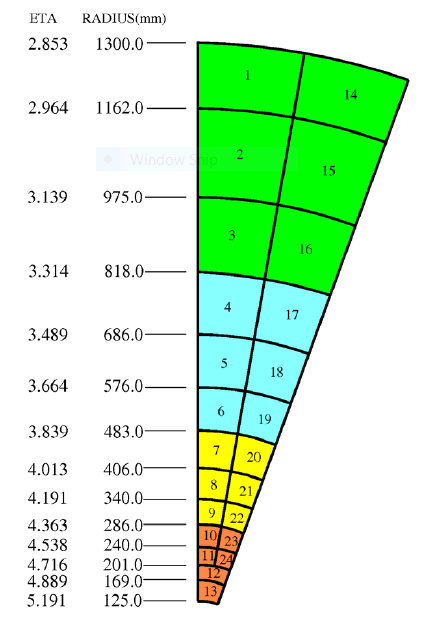
\includegraphics[scale=0.5]{Chapter2/hfes.PNG}
    \caption[Hadron forward wadge.]{And r-$\phi$ view of a HF wadge.}
    \label{wedge}
\end{figure}
\end{center}
\subsection{Muon Detector}
The last subdetector of the CMS experiment is the muon detector system located in the magnet return yokes. The muon system consists of 3 types of gaseous detectors, used to detect muons and their momenta. These detectors are:  the drift tube chambers (DT), the cathode strips chambers (CSC) and the resistive plate chamber (RPC). These detector are distributed across the 2 central parts of the muon detector, the barrel and endcap sessions, with a coverage of $|\eta|<1.2$ and $|\eta|<2.4$ respectively. The distribution of these detectors is shown in Figure \ref{Muons}.
\begin{figure}[H]
    \centering
    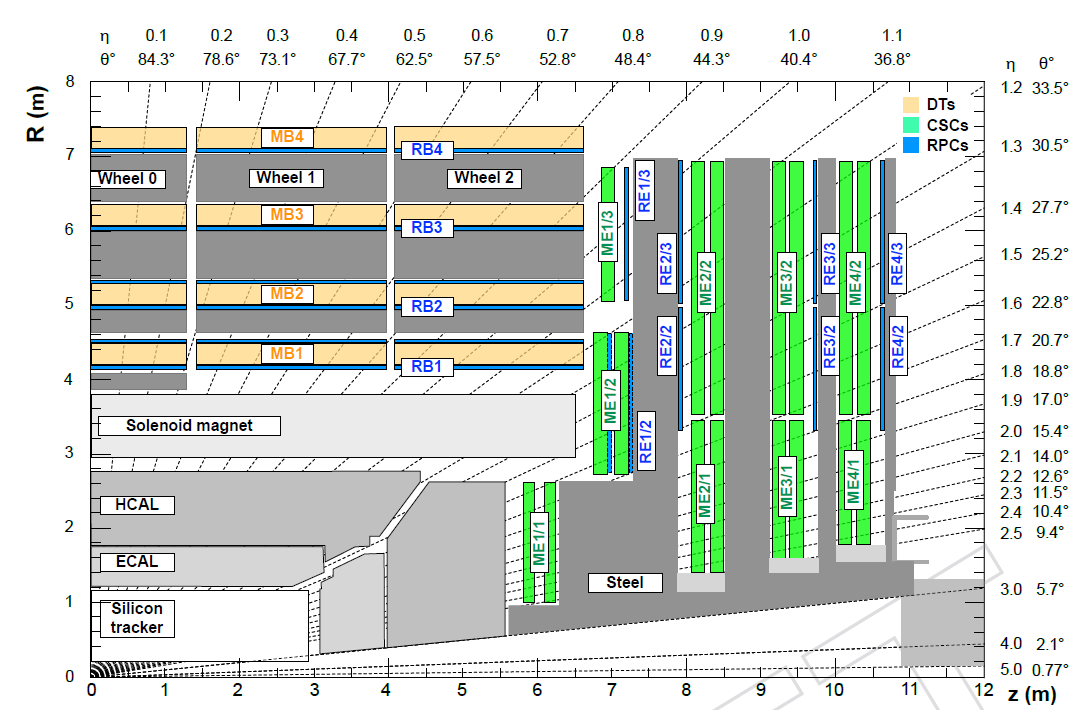
\includegraphics[scale=.45]{Chapter3/dt.png}
    \caption[One quarter of the CMS muon system. ]{The diagram shows the layout of one quarter of the muon system at CMS \cite{cms-manual}.}
    \label{Muons}
\end{figure}

The barrel DT detector  has a coverage of $|\eta|<1.2$, and consist of 250 chambers arranged in 4 layers inside the magnet return yoke, at a radii of approximately 4, 4.9, 5.9 and 7 meters from the beam line. The basic element of the DT detectors are cells, with a transverse size of $42\times 13$ $mm^2$, filled with a gas mixture of $85\%$ Ar and $15\%$ $CO_2$ \cite{cms7}. The cells have a gold-plated stainless steel anode wire, connected at their center. The wire has a diameter of 50 $\mu m$ and it operates at a voltage of +3600 V. \\
The barrel detectors are divided into 12 sectors, each covering $30^{\circ}$ in the azimuthal direction.

Installed on the encap regions, the CSC chambers are installed, covering a range of $0.9<\eta<2.4$. Their fast response time and their tolerance to non-uniform magnetic fields, makes the perfect for the high muon rates and background levels found in this region. The 6 layers of the CSC measure the muon positions in 2 coordinates. The cathode strips provide precise measurements on the r-$\phi$ bending plane, while the wires provide a coarse measurement in the radial direction. Each layer of the CSC contains 80 cathode strips with anode wires, of diameter 50 $\mu m$, running almost parallel to the cathodes.\\
In total, the 2 encaps are comprised of 468 CSC chambers, filled with a gas mixture of $50\%$ $CO_2$, $40\%$ Ar and $10\%$ $CF_4$ \cite{cms7}.

The RPC detectors is located in the barrel and encap regions of the muons system, complementing the DT and CSC detectors. It covers a region of $|\eta|<1.6$ and it provides fast, independent trigger events. The RPC are double-gap chambers, each gap consisting of 2 mm thick resistive bakelite plates, separated by a 2 mm thick gas gap.  Readout strips are aligned in the $\eta$ direction in between the gas gaps. The gaps are filled with a gas mixture of $95.2\%$ Freon $(C_2H_2F_4)$, $4.5\%$ isobutane $(i-C_4H_{10})$, and $0.3\%$ sulphur hexafluoride $(SF_6)$. Water vapor is added to reach a mixture humidity of $40\%$-$50\%$ \cite{cms7}. 



%%%%%%%%%%%%%%%%%%%%%%%%%%%%%%%%%%%%%%%%%%%%%%%%%%%%%%%%%%%%%%%%%%%%%%%%%%%%%%%%%%%

\section{High Luminosity LHC}
The LHC is the most powerful particle collider in the world, and it is to remain the most powerful for the next two decades. To ensure this, the LHC will receive major upgrades during the 2020s, to increase its luminosity by a factor of 5 beyond the original design. About 10 years will be needed to study and prototype the technologies required for the new High Luminosity LHC (HL-LHC). The HL-LHC project was created at the end of  2010 by CERN, as a response to the  European strategy for particle physics, to fully exploit the capabilities of the LHC. The project was approved on 30 of May of 2013 by the CERN council in charge at the time. For the next decade the HL-LHC is the major construction project of CERN. Several new technologies will be used to achieve the luminosity goal, some of them include: superconducting magnets capable of producing a magnetic field of 11 to 12 T, superconducting  cavities, compact and with phase control, for beam rotation, long high-power superconducting links with zero energy dissipation and new technologies for beam collimation \cite{cern3}.
\begin{center}
\begin{figure}[H]
    \centering
    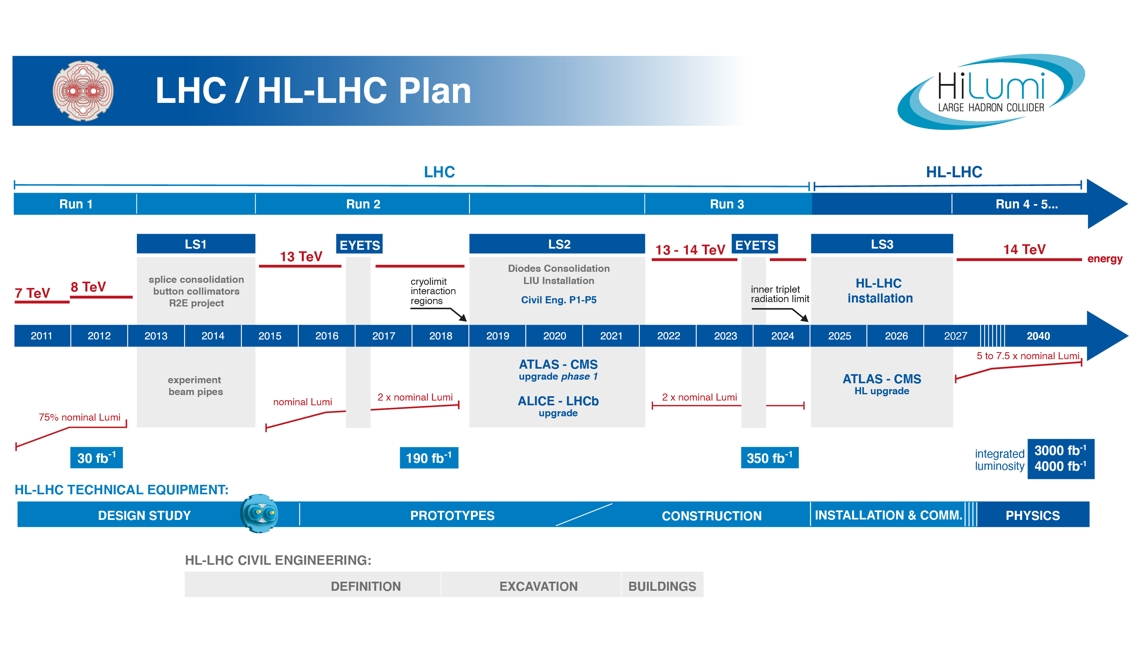
\includegraphics[scale=1.5]{Chapter2/schedulelhc.jpg}
    \caption[schedule of the LHC.]{The past and future schedule of the LHC. The red line corresponds to the center-of-mass-energy of the pp collisions, while the light-red line shows the expected luminosity \cite{schedule}.}
    \label{programing}
\end{figure}
\end{center}
Figure \ref{programing} shows the  schedule of the LHC up until 2025, where the new phase of the LHC, the HL-LHC, will  begin. After reaching a center-of-mass-energy of 13 during 2015, the LHC has doubled the luminosity for which it was designed, as  of the end of Run 2.

The main objectives of the HL-LHC is to reach a peak luminosity of 5 to $7.5\times10^{34}$ $cm^{-2}s^{-1}$, and an integrated luminosity of 250 $fb^{-1}$ per year, with the goal of reaching a total integrated luminosity of 3000 $fb^{-1}$, in the first 12 years of the machines operation. For this, intensive studies have, and are, being conducted to determine the hardware and the configuration needed to achieve these goals.\\
The new hardware of the HL-LHC is to be installed during the third long shutdown (LS3). To ensure that the integrated luminosity goal is met, all equipment is being designed with a $50\%$ margin in regards to the required luminosity. This means that the High Luminosity LHC can reach peak luminosity valued of 7 to $7.5\times10^{34}$ $cm^{-2}s^{-1}$, this will mean an increase in total pileup (rate of pp collision per bunch crossing) up to 200 \cite{cern3}.




%%%%%%%%%%%%%%%%%%%%%%%%%%%%%%%%%%%%%%%%%%%%%%%%%%%%%%%%%%%%%%%%%%%%%%%%%%%%%%%%%%%
\section{Tracker End-Cap Pixel luminometer}

Along with the new HL-LHC upgrade, several upgrades will come to the CMS detector to accommodate the new luminosity and pileup requirements.  The tracker, muon end caps, trigger and beam radiation protection are just a few of the new upgrades scheduled for the CMS detector. However, the focus of this work will be solely on the tracker upgrades, more specifically, the inner  tracker end cap pixel (TEPX) luminometer.

For Phase-2 of the CMS tracking the entire existing pixel and strip tracker will be replaced. Figure \ref{TEPXl} shows the r-z layout of the three sections of the Phase-2 inner tracker: the  tracker barrel pixel (TBPX), composed of four cylindrical layers of modules, the tracker’s forward (TFPX) and the tracker end-cap (TEPX) pixel detectors, made of 8 and 4 disks of pixel modules respectively. The new tracker will include: increased granularity, forward acceptance and radiation hardness as well as compatibility with longer trigger latency and higher data rates.
The silicon pixel modules will have a thickness of 100-150 $\mu m$, while the pixel cells will have an area of 2500 $\mu m^2$ ($25\times 100$ $\mu m^2$) \cite{CERN-LHCC-2017-009}\cite{DelBurgo:2706637}. Two types of modules will be used in the inner tracker, modules with 2 and 4 pixel chips. The modules will be arranged in $2\times1$ and $2\times 2$, these modules are depicted as green and yellow respectively in  Figure \ref{TEPXl}. TBPX and TFPX will be composed of both types of modules, while TEPX will only use $2\times 2$ modules \cite{DelBurgo:2706637}. 
\begin{center}
\begin{figure}[H]
    \centering
    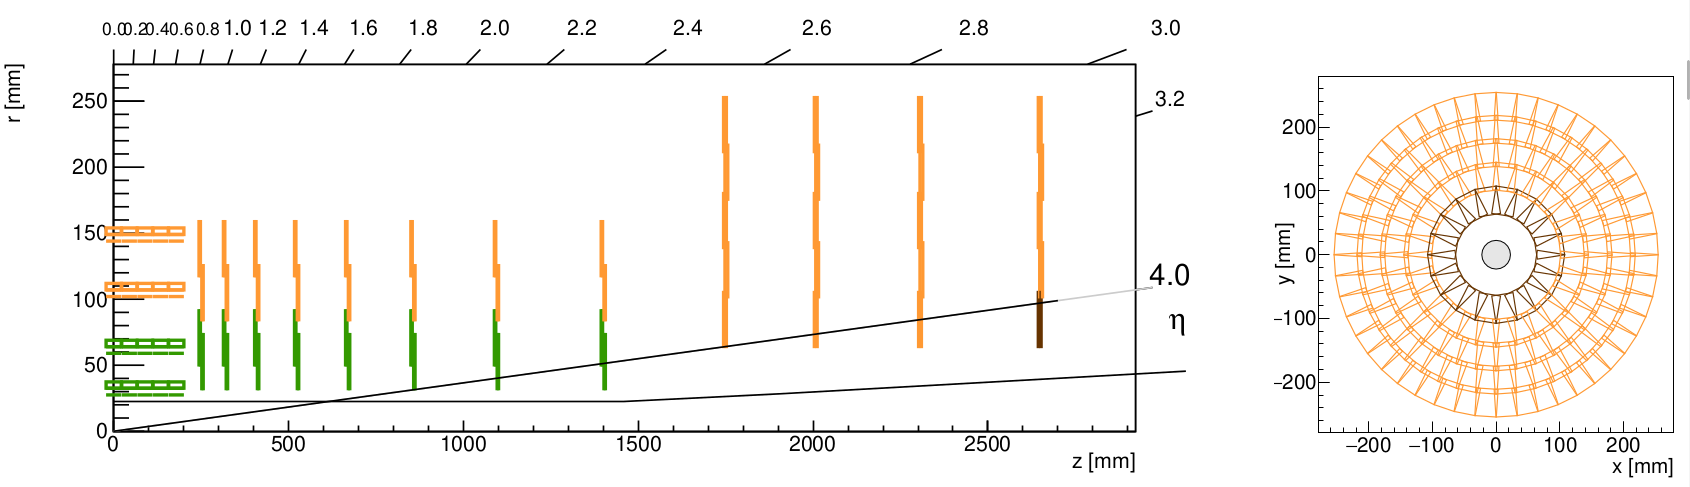
\includegraphics[scale=.2]{Chapter2/TEPX.png}
    \caption[Diagram of the Phase-2 inner tracker upgrade.]{\textit{Lefts}: Diagram of the Phase-2 inner tracker upgrade. The last four yellow lines between 1700 mm and 2700 mm, correspond to the TEPX subdetector. \textit{Right}:  Front view of one of the disks of the TEPX subdetector \cite{DelBurgo:2706637}.}
    \label{TEPXl}
\end{figure}
\end{center}
For Phase-2 the TEPX portion of the tracker will be designated for tracking and luminosity measurements, while disk 4 ring 1 (TEPXD4R1) of the detector will designated for luminosity measurements only. The TEPX detector is located at each extremity of the tracker of the CMS detector, with a range  from 175 cm to 265 cm on the $|z|$ direction and a radius  between 63 mm and 255 mm. The detector is composed of 4 double sided disks, each one made of 5 concentric rings of pixel modules. To guarantee hermetic coverage, each ring has a different number of pixel modules. TEPX is composed of 800 million pixels, distributed over an area of 2$m^2$, and will operate at trigger frequency of 75KHz during physics runs. Table \ref{rings} shows the number of modules per ring, as well as the radius of each ring.

\begin{table}[H]
\centering
\caption[Radius and number of pixel modules that comprise the rings of the TEPX subdetector.]{ Table shows the inner ($r_{in}$) and outer ($r_{out}$) radius, as well as the number of pixel modules that comprise each ring of each disk of the TEPX subdetector}
\scalebox{.8}{
\begin{tabular}{|l | c | c | c |c|c|}
\hline
 Ring & 1& 2&3&4&5   \\
\hline
$r_{in}$ (mm) & 62.9&100.55 &137.85 &174.45 &210.5\\
\hline
$r_{out}$ (mm)&107.69 &144.99 &182.09 &218.56 &254.51 \\
\hline
 No. of modules&20 &28 &36 &44&48 \\
\hline
\end{tabular}}
\label{rings}
\end{table}


The innermost ring of the last disk, disk 4 ring 1 (TEPXD4R1), lies beyond a pseudorapidity of $|\eta|=4$ and due to the low number of tracking points in this region, this ring will be designated for luminosity measurements only. The ring consists of 20 modules, and it has an inner radius of 62.9 mm and an outer radius of  107.69 mm. Finally, the luminometer may run at a trigger frequency of 825kHz to several MHz.\\
Luminosity measurements with the TEPX's detectors will be carried out using the Pixel cluster counting (PCC) method described in the next chapter.
